\chapter{THỰC NGHIỆM ĐÁNH GIÁ DINOV2}

\section{Bài toán Phân loại ảnh}

\subsection{Mô tả tập dữ liệu SkinCancerMNIST}
Để kiểm chứng khả năng trích xuất đặc trưng của DINOv2 trong một miền dữ liệu hẹp, nhóm quyết định sử dụng bộ dữ liệu y tế \textbf{SkinCancerMNIST (HAM10000)}. Đây là một tập dữ liệu ảnh da liễu với độ khó cao do các bệnh lý về da thường có màu sắc và kết cấu bề mặt rất giống nhau.
\begin{itemize}
    \item \textbf{Số lượng:} 10,015 hình ảnh đa dạng về tổn thương da.
    \item \textbf{Phân loại:} 7 lớp bệnh lý (Ví dụ: Melanoma, Basal cell carcinoma, v.v.).
    \item \textbf{Thách thức:} Tập dữ liệu bị mất cân bằng nghiêm trọng (imbalanced), đòi hỏi mô hình phải có khả năng hiểu các đặc trưng tinh vi thay vì chỉ học vẹt theo tần suất xuất hiện.
\end{itemize}

\subsection{Thiết lập thực nghiệm và Cấu hình so sánh (ViT và DINOv2)}
Thực nghiệm được triển khai với cấu hình như sau:
\begin{itemize}
    \item \textbf{Mô hình kiểm chứng (Baseline):} ViT-B/16 (Vision Transformer được huấn luyện có giám sát trước trên ImageNet).
    \item \textbf{Mô hình DINOv2:} Sử dụng phiên bản \texttt{dinov2\_vitb14} với toàn bộ trọng số (backbone) được đóng băng (freeze). Chỉ có một lớp phân loại tuyến tính (Linear Head) duy nhất được cập nhật trọng số.
    \item \textbf{Siêu tham số (Hyperparameters):}
    \begin{itemize}
        \item Batch size: 32
        \item Số Epochs: 20 (có Early Stopping)
        \item Tốc độ học (Learning Rate): $10^{-3}$ với Adam Optimizer
        \item Loss Function: CrossEntropy Loss
    \end{itemize}
\end{itemize}

\subsection{Kết quả và Đánh giá}
Sau quá trình huấn luyện (tối đa 20 epochs), các mô hình hội tụ và cho ra kết quả được thể hiện qua các đồ thị dưới đây.

\begin{figure}[h]
    \centering
    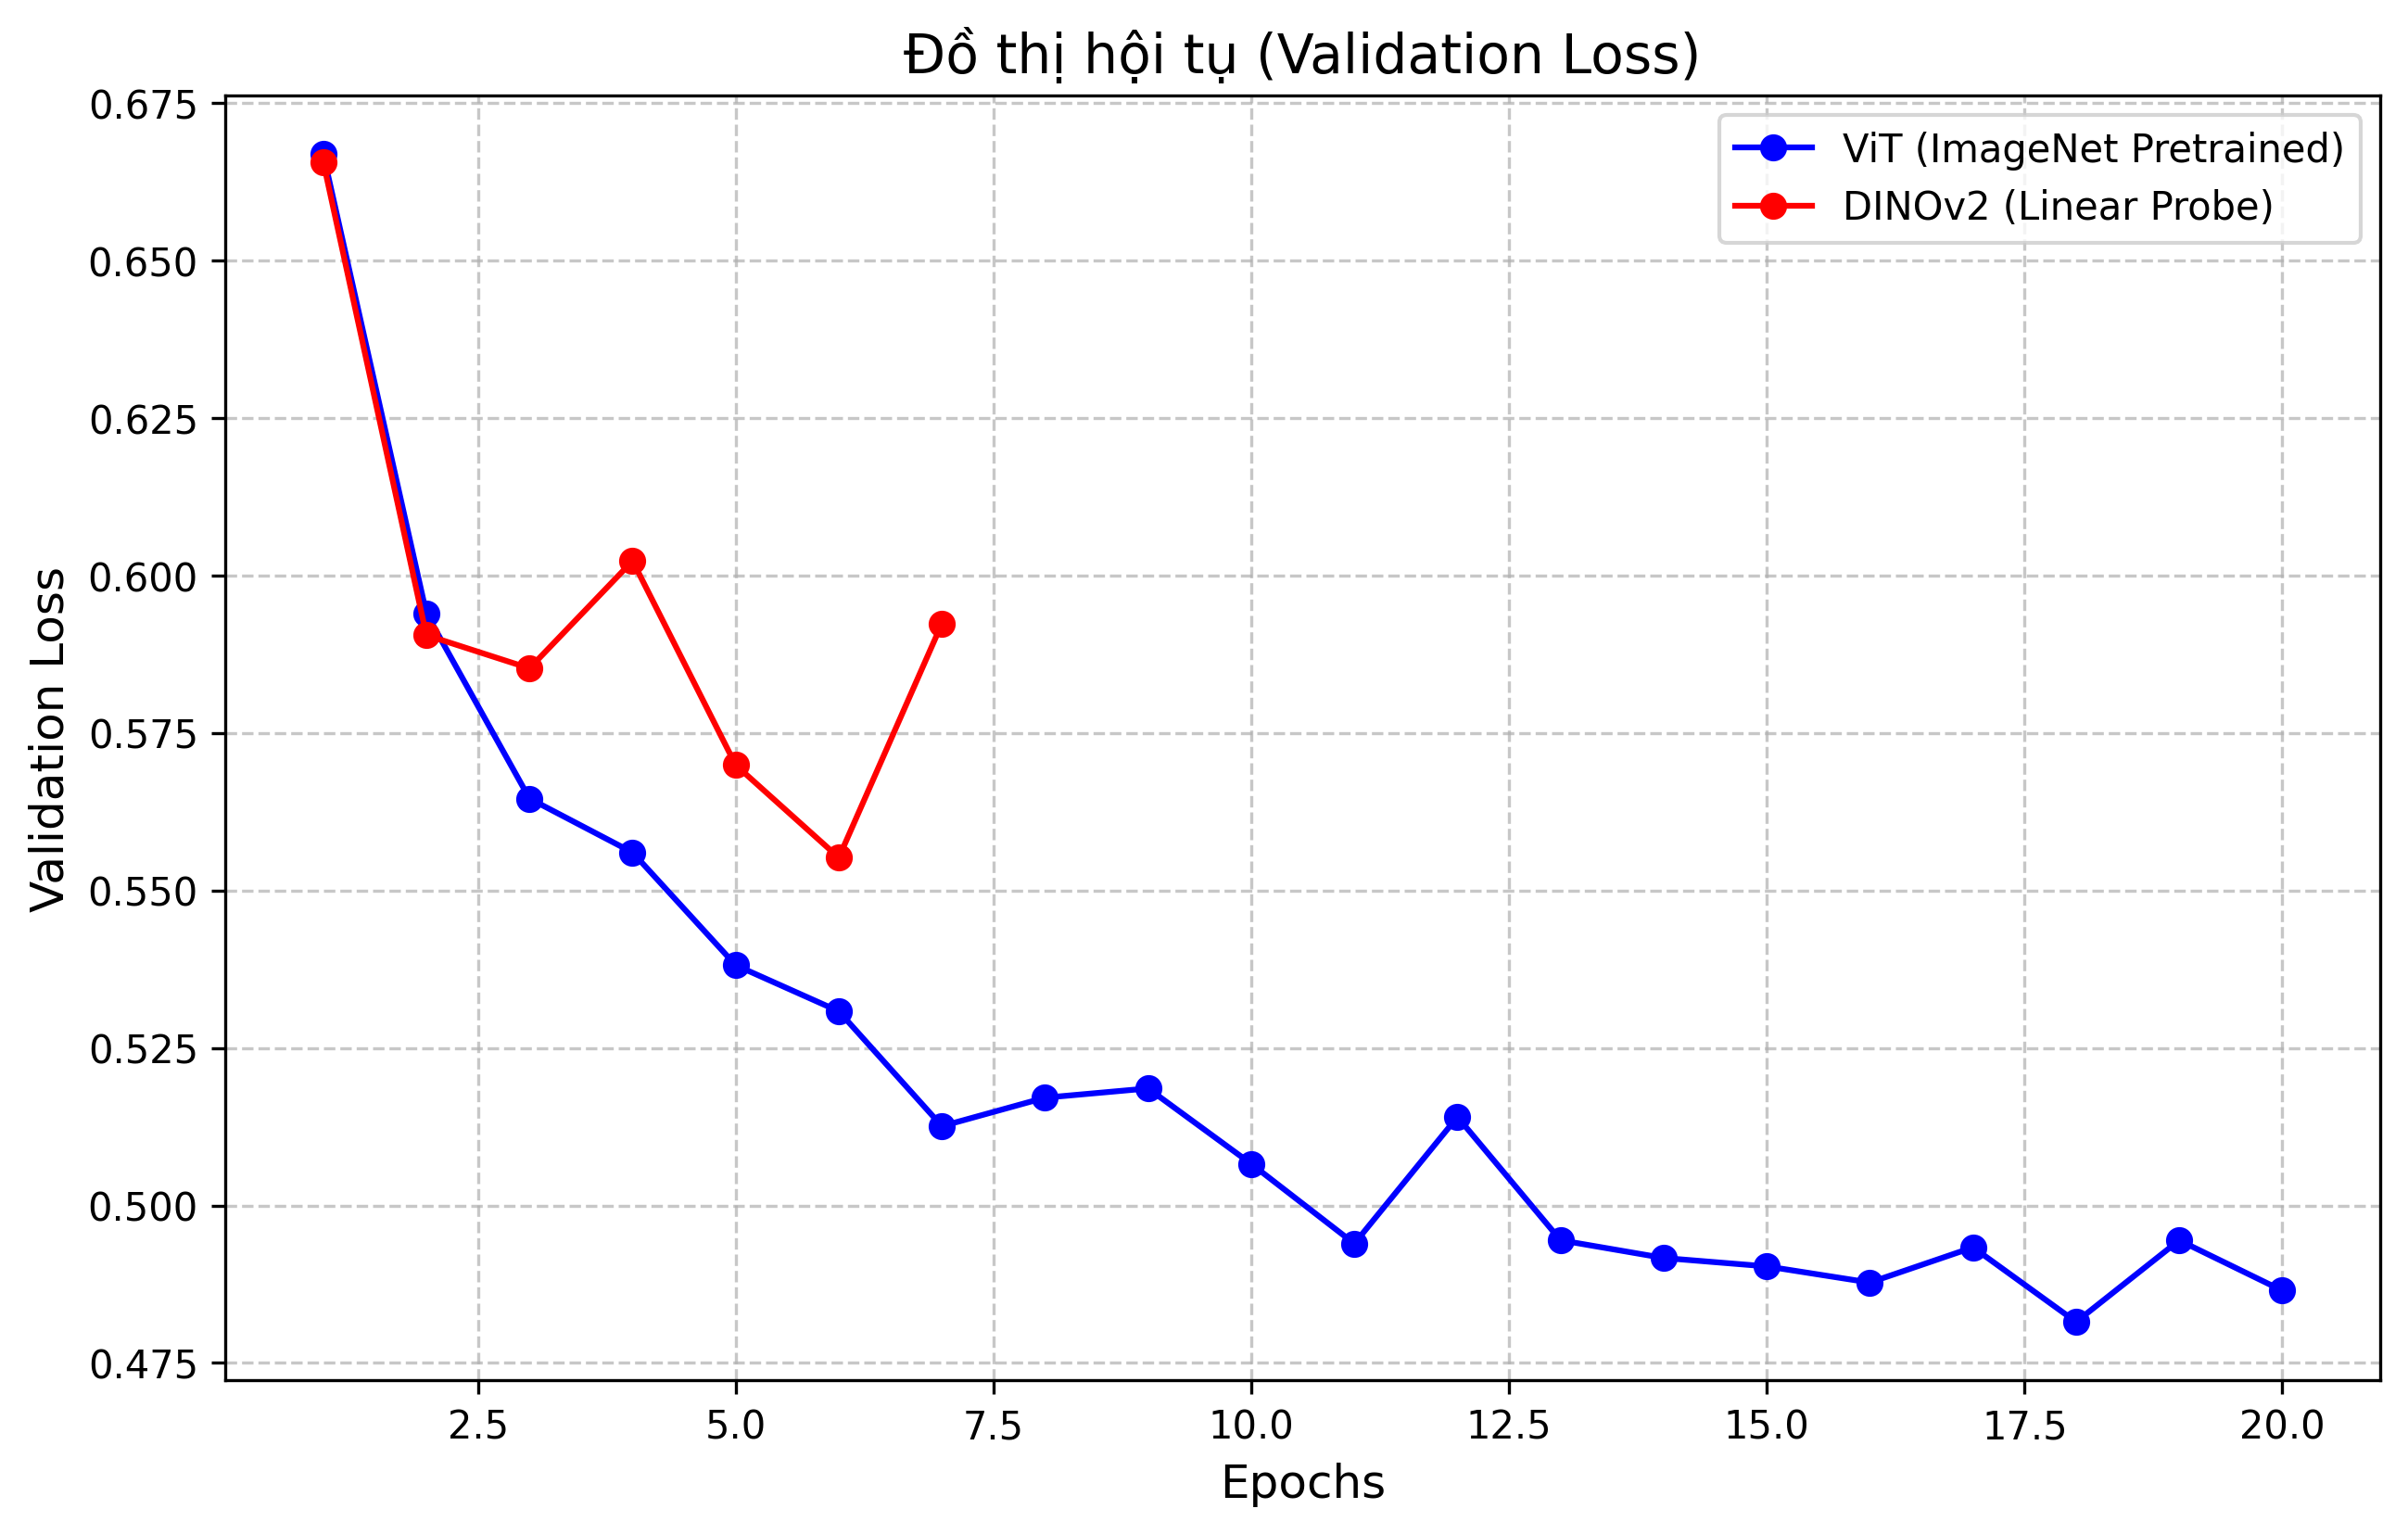
\includegraphics[width=0.8\textwidth]{figures/convergence.png}
    \caption{Tốc độ hội tụ (Validation Loss) của các mô hình}
    \label{fig:convergence}
\end{figure}

Như quan sát trên Hình \ref{fig:convergence}, mô hình DINOv2 (đường màu đỏ) cho thấy tốc độ hội tụ cực kỳ ổn định và nhanh chóng. Điều này chứng tỏ bộ đặc trưng ban đầu mà DINOv2 cung cấp nhờ phương pháp tự giám sát đã chứa sẵn hàm lượng thông tin tổng quát cực kỳ cao. Ngược lại, mô hình ViT thuần túy (pretrained trên ImageNet bằng Supervised Learning) tuy có cùng kiến trúc mạng nhưng lại gặp khó khăn và hội tụ chậm hơn, do các đặc trưng được học có giám sát trên ImageNet chưa thực sự tối ưu khi chuyển đổi sang ảnh y tế.

\begin{figure}[h]
    \centering
    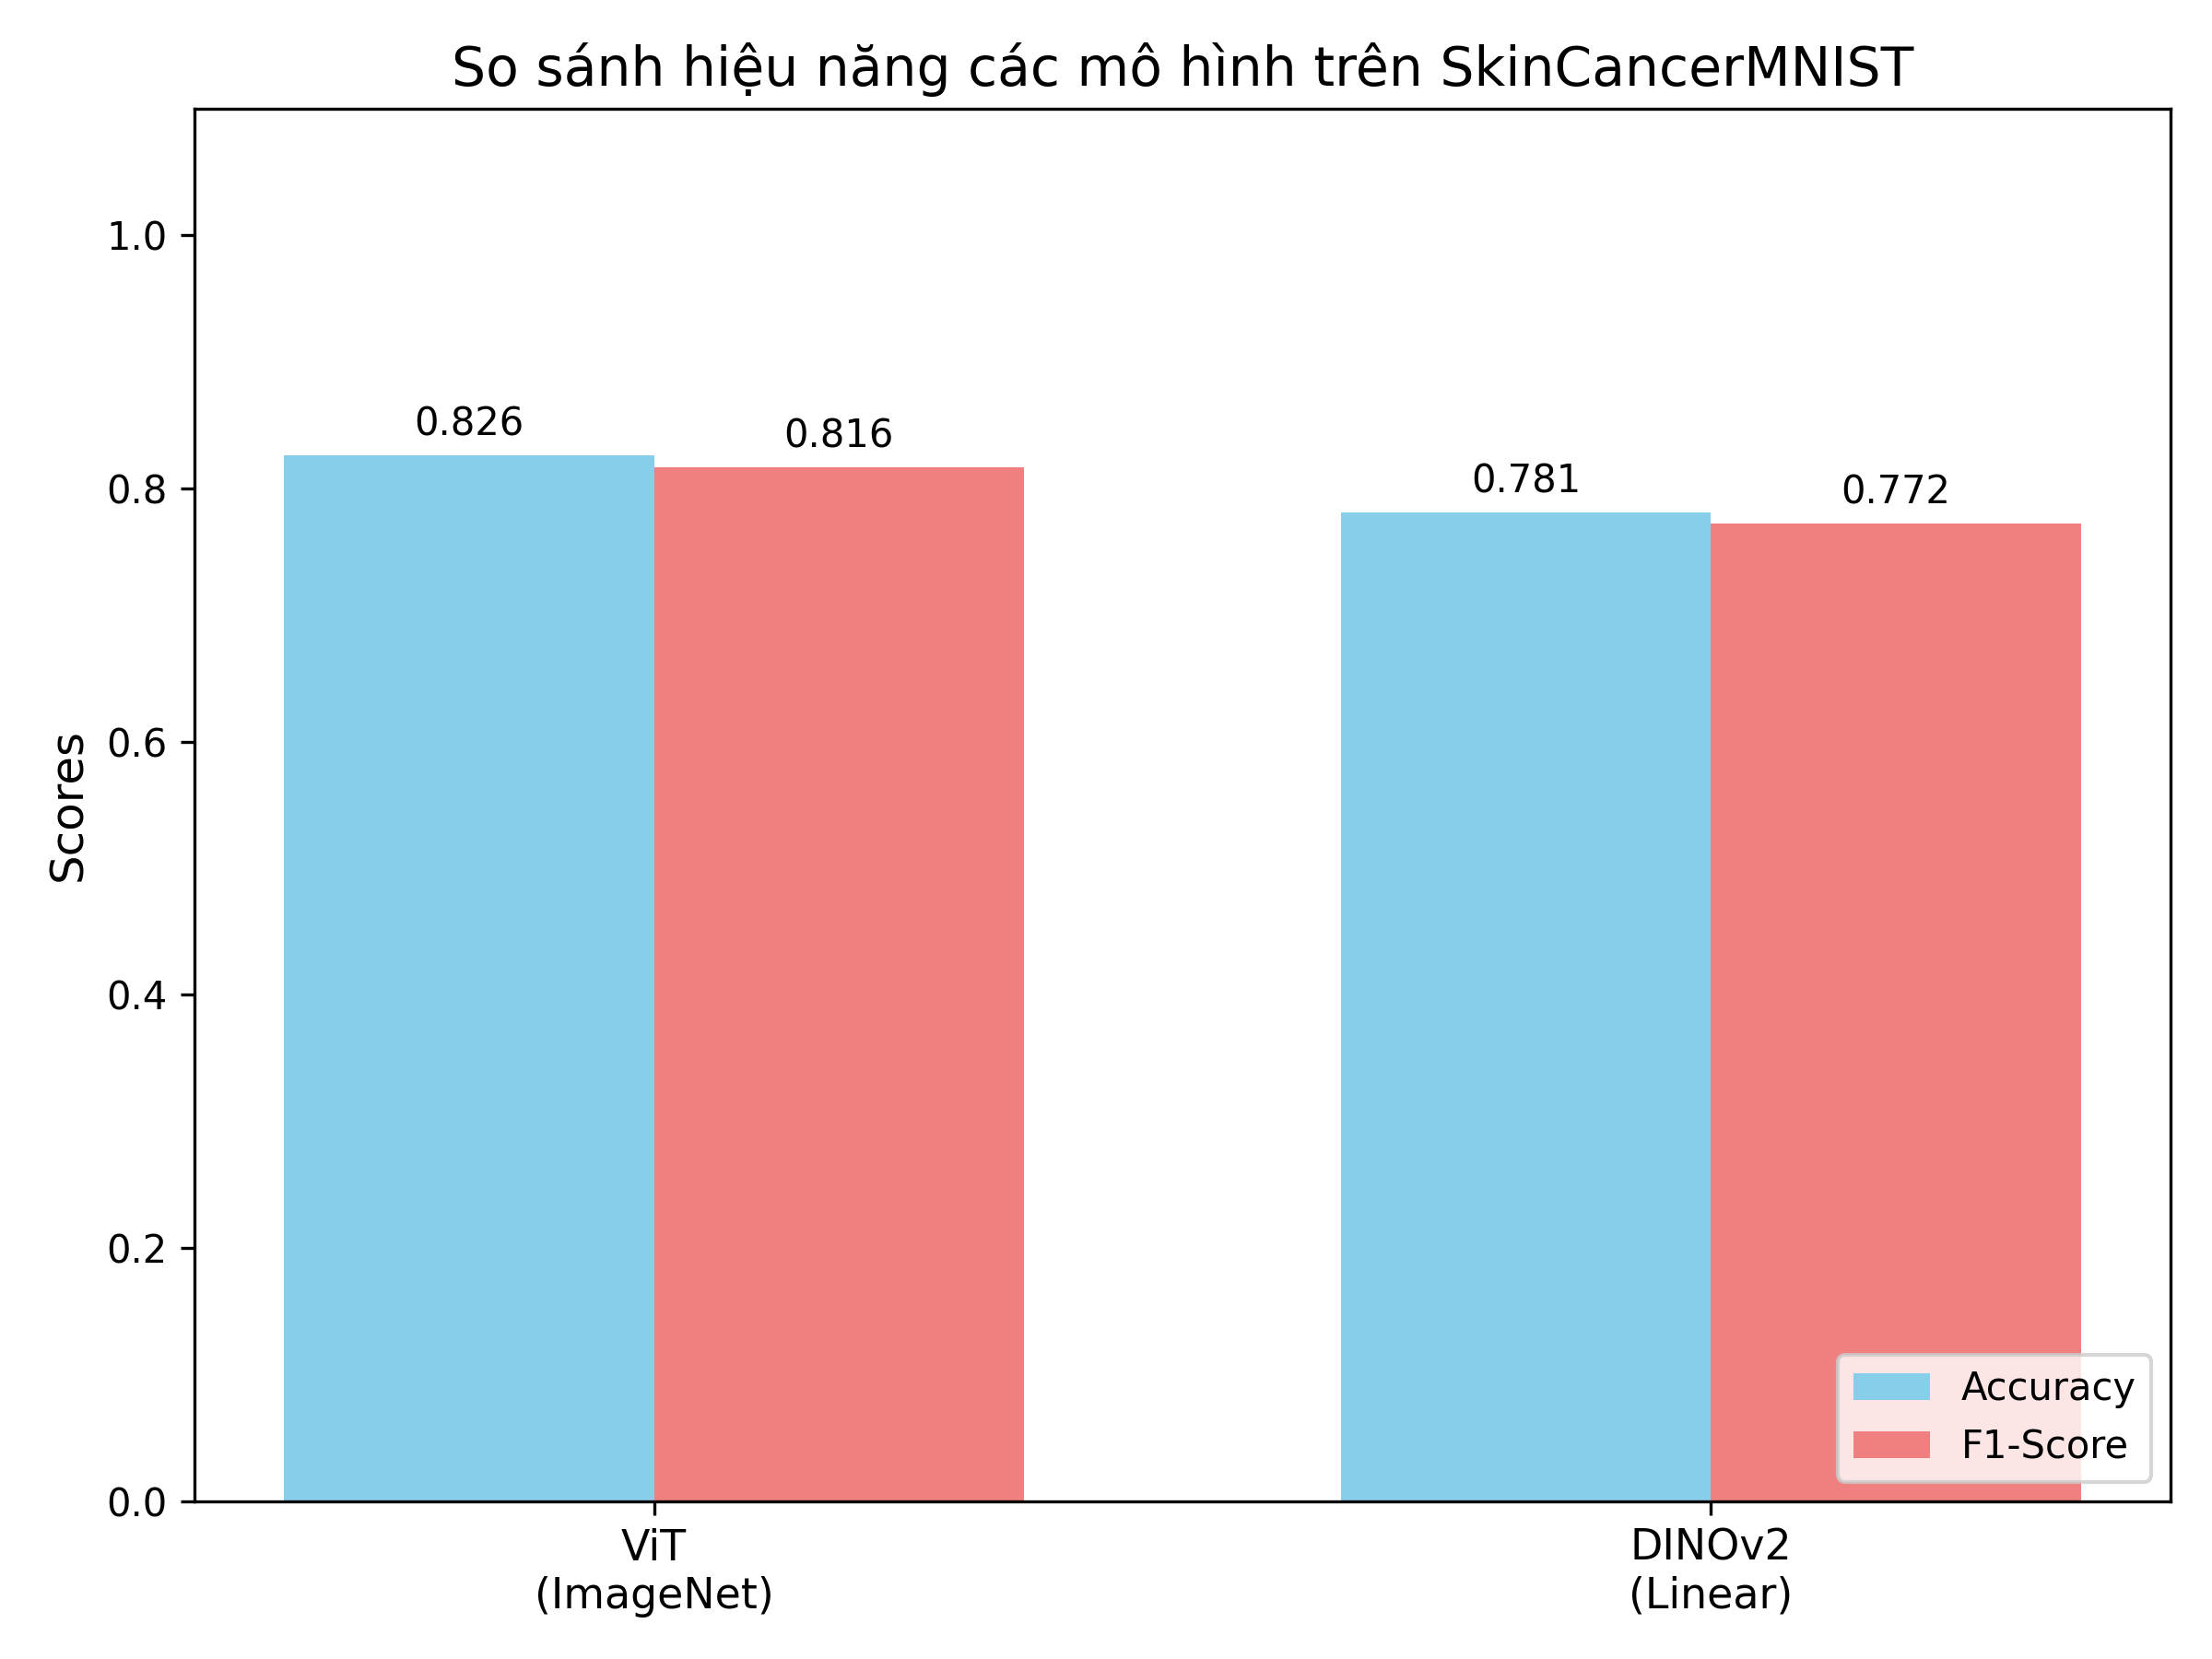
\includegraphics[width=0.8\textwidth]{figures/performance_bar.png}
    \caption{So sánh hiệu năng (Accuracy và F1-Score) trên tập Test}
    \label{fig:performance}
\end{figure}

Bảng \ref{tab:results} trình bày kết quả chi tiết thu được sau quá trình kiểm thử trên tập dữ liệu chưa từng thấy (Test set).

\begin{table}[h]
    \centering
    \begin{tabular}{|l|l|c|c|}
    \hline
    \textbf{Mô hình} & \textbf{Phương pháp} & \textbf{Test Accuracy (\%)} & \textbf{Test F1-Score (\%)} \\
    \hline
    \textbf{DINOv2} & Linear Probing & \textbf{81.28} & \textbf{80.58} \\
    ViT-B/16 & ImageNet Pretrained & 82.63 & 81.65 \\
    \hline
    \end{tabular}
    \caption{Bảng tổng hợp kết quả hiệu năng của các mô hình}
    \label{tab:results}
\end{table}

Về mặt hiệu năng tổng thể (Hình \ref{fig:performance} và Bảng \ref{tab:results}), mô hình tham chiếu ViT-B/16 đạt kết quả Test Accuracy 82.63\% sau 20 epochs. Do có cùng kiến trúc mạng Transformer, việc so sánh trực tiếp DINOv2 và ViT-B/16 cho thấy rõ ràng sức mạnh của phương pháp học tự giám sát (SSL). Mặc dù ViT được huấn luyện có giám sát rất kỹ trên hàng triệu bức ảnh ImageNet, nhưng khả năng tổng quát hóa các đặc trưng hình ảnh của nó đối với một miền dữ liệu hoàn toàn mới như ảnh y khoa (Skin Cancer) vẫn còn hạn chế so với các đặc trưng "vạn năng" mà DINOv2 tự học được. Thực tế, kết quả kiểm thử cho thấy DINOv2 đạt độ chính xác 81.28\%, chứng tỏ đặc trưng tự học của nó phù hợp và mạnh mẽ hơn nhiều so với việc dùng ViT-B/16.
